Business Process Model and Notation (BPMN) ist eine Standard-Notation, um Geschäftsprozesse zu modellieren, welche von allen Teilnehmern verstanden werden können. Die aktuelle Version 2.0 des Standards wurde 2011 von der Object Management Group (OMG) entwickelt. Prozesse bestehen aus einer Abfolge von Flow-Elementen. Diese Flow-Elemente sind durch Sequenzflüsse miteinander verbunden, welche den Ablauf des Prozesses vorgeben. Der Umfang von Prozessen kann von Aufgaben für eine Person hin zu firmenweiten Tätigkeiten reichen \cite{omgbpmn}.

Ein Ziel der OMG ist es, eine Brücke zwischen der Modellierung und der Implementierung zu schaffen. Der Standard kann im Dialog zwischen Geschäftspartnern jeder Ebene als schnelle Anforderungsübersicht dienen, den Entwicklern helfen, die Geschäftsprozessen zu implementieren und im Anschluss das Überwachen und Warten erleichtern. Ein anderes Ziel von BPMN 2.0 ist es, Prozesse visualisieren zu können, welche durch eine zur Ausführung entworfene XML Sprache modelliert sind \cite{omgbpmn}.

In der BPMN 2.0 Spezifikation werden drei Unterprozesstypen beschrieben: Konversationsdiagramme, Kollaborationsdiagramme und Prozessdiagramme.
Konversationsdiagramme modellieren die Logik vom Nachrichtenaustausch. Kollaborationsdiagramme beschreiben die Interaktion von verschiedenen Prozessteilnehmern. Prozessdiagramme sind für den Prozessablauf von Aktivitäten da und werden in der BPMN als Graph dargestellt \cite{omgbpmn}. In dieser Arbeit wird mit Prozessdiagrammen gearbeitet. Nachfolgend folgt eine Erklärung aller für diese Arbeit relevanten Flow-Elemente.

\section{Aktivitäten}

Eine Aktivität ist eine Tätigkeit, welche innerhalb von einem Geschäftsprozess ausgeführt wird. Es gibt drei Arten von Aktivitäten: Aufgabe, Subprozess und das Aufrufen von einer anderen Aktivität. Eine Aufgabe ist eine kleinste mögliche atomare Aktivität, welche meist von einem Benutzer ausgeführt wird. Sie wird durch ein abgerundetes Rechteck abgebildet (siehe Abbildung \ref{fig:activities}).
Eine Aufgabe kann zudem einen Typen zugewiesen bekommen. Dieser wird oben links im Rechteck durch ein passendes Symbol dargestellt. Diese Eigenschaft wird im weiteren Verlauf der Arbeit für die Gamifizierung noch interessant werden \cite{omgbpmn}.

\phantomsection
\begin{figure}[ht]
    \centering
    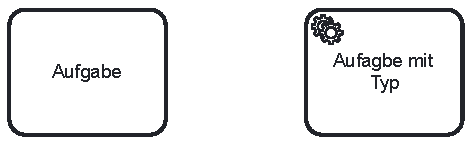
\includegraphics[width=.5\textwidth]{images/activities}
    \caption{Aufgabe ohne und Aufgabe mit Typ}
    \label{fig:activities}
\end{figure}

\section{Datenobjekte und Assoziationen}

Mithilfe von Datenobjekten können Informationen im Laufe des Prozesses geladen und gespeichert werden. Assoziationen ermöglichen es, Informationen zwischen Datenobjekten und Aktivitäten zu transportieren. Sie haben keinen Einfluss auf den Prozessablauf. Datenobjekte werden durch eine Notiz und Assoziationen durch einen gestrichelten Pfeil mit offener Spitze dargestellt (siehe Abbildung \ref{fig:data_object_association}). Die Informationen werden in Richtung des Pfeils transportiert \cite{omgbpmn}.

\phantomsection
\begin{figure}[ht]
    \centering
    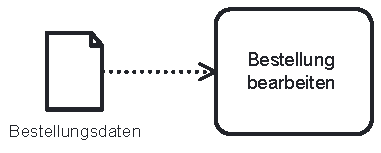
\includegraphics[width=.4\textwidth]{images/data_object_association}
    \caption{Datenobjekt mit Assoziation zu einer Aufgabe}
    \label{fig:data_object_association}
\end{figure}

\section{BPMN 2.0 XML}

BPMN 2.0 XML ist eine Auszeichnungssprache, welche auf einer von OMG erstellten XML Schema Definition (XSD) basiert \cite{omgbpmn-xsd}. Sie dient dazu, BPMN 2.0 Modelle abzuspeichern und somit einen Austausch zwischen unterschiedlichen Anwendungen zu ermöglichen. Eine BPMN 2.0 XML Datei hat die Endung \emph{.bpmn} \cite{omgbpmn}.